\documentclass{article}
\usepackage{tikz, comment}
\usepackage{pifont}
\usepackage{fontspec}
\usetikzlibrary{arrows, decorations.markings, decorations.pathreplacing}
\begin{comment}
:Title: Not defined yet
:Tags: symmetric;curves;curve
:Author: Prof.Hu Ji-shan, HKUST
:Slug: No name yet

Description Here.........
\end{comment}
\begin{document}\centering

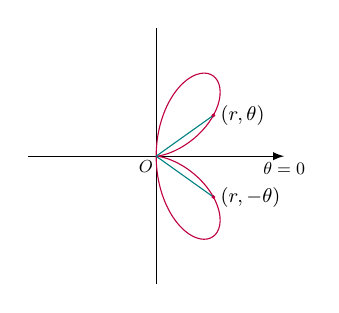
\begin{tikzpicture}[>=latex,xscale=.5*0.65, yscale=.5*0.65][font=\sf\small]

\draw[->] (-5, 0) -- (5, 0)node[below, scale=0.7] {$\theta=0$};
\draw[] (0, -5) -- (0, 5);

\draw[purple, samples=100, smooth, domain=0:1*pi, variable=\t]
plot ({10*(sin((1*\t) r))^2*1*cos((1*\t) r)*cos(\t r)}, {10*(sin((1*\t) r))^2*1*cos((1*\t) r)*sin(\t r)}) ;

\draw[teal] (0,0)--({10*(sin(0.62 r))^2*1*cos(0.62 r)*cos(0.62 r)}, {10*(sin(0.62 r))^2*1*cos(0.62 r)*sin(0.62 r)});
\draw[teal] (0,0)--({10*(sin(-0.62 r))^2*1*cos(-0.62 r)*cos(-0.62 r)}, {10*(sin(-0.62 r))^2*1*cos(-0.62 r)*sin(-0.62 r)});

\draw[purple, fill] ({10*(sin(0.62 r))^2*1*cos(0.62 r)*cos(0.62 r)}, {10*(sin(0.62 r))^2*1*cos(0.62 r)*sin(0.62 r)}) circle(0.05) node[black, right, scale=0.8] {$(r, \theta)$};
\draw[purple, fill] ({10*(sin(-0.62 r))^2*1*cos(-0.62 r)*cos(-0.62 r)}, {10*(sin(-0.62 r))^2*1*cos(-0.62 r)*sin(-0.62 r)}) circle(0.05) node[black, right, scale=0.8] {$(r, -\theta)$};

\node[scale=0.7] at (-0.3/0.75, -0.3/0.75) {$O$};

\end{tikzpicture}\hskip0.5cm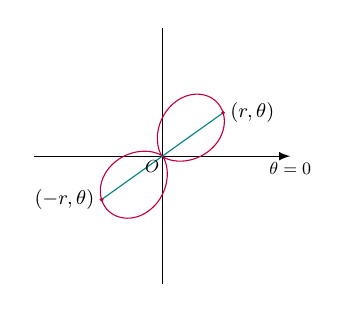
\begin{tikzpicture}[>=latex,xscale=.5*0.65, yscale=.5*0.65][font=\sf\small]

\draw[->] (-5, 0) -- (5, 0)node[below, scale=0.7] {$\theta=0$};
\draw[] (0, -5) -- (0, 5);

\draw[purple, samples=100, smooth, domain=0:2*pi, variable=\t]
plot ({1.5*(1*sin((1*\t) r) + 1*cos((1*\t) r))^2*cos(\t r)}, {1.5*(1*sin((1*\t) r) + 1*cos((1*\t) r))^2*sin(\t r)}) ;

\draw[teal] (0,0)--({1.5*(1*sin(0.62 r) + 1*cos(0.62 r))^2*cos(0.62 r)}, {1.5*(1*sin(0.62 r) + 1*cos(0.62 r))^2*sin(0.62 r)});
\draw[teal] (0,0)--({-1.5*(1*sin(0.62 r) + 1*cos(0.62 r))^2*cos(0.62 r)}, {-1.5*(1*sin(0.62 r) + 1*cos(0.62 r))^2*sin(0.62 r)});

\draw[purple, fill] ({1.5*(1*sin(0.62 r) + 1*cos(0.62 r))^2*cos(0.62 r)}, {1.5*(1*sin(0.62 r) + 1*cos(0.62 r))^2*sin(0.62 r)}) circle(0.05) node[black, right, scale=0.8] {$(r, \theta)$};
\draw[purple, fill] ({-1.5*(1*sin(0.62 r) + 1*cos(0.62 r))^2*cos(0.62 r)}, {-1.5*(1*sin(0.62 r) + 1*cos(0.62 r))^2*sin(0.62 r)}) circle(0.05) node[black, left, scale=0.8] {$(-r, \theta)$};

\node[scale=0.7] at (-0.3/0.75, -0.3/0.75) {$O$};

\end{tikzpicture}\hskip0.5cm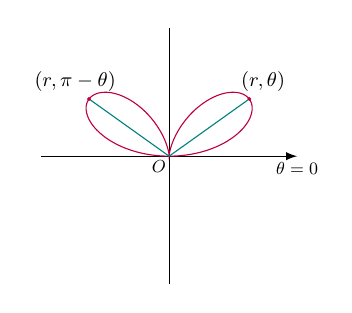
\begin{tikzpicture}[>=latex,xscale=.5*0.65, yscale=.5*0.65][font=\sf\small]

\draw[->] (-5, 0) -- (5, 0)node[below, scale=0.7] {$\theta=0$};
\draw[] (0, -5) -- (0, 5);

\draw[purple, samples=100, smooth, domain=0:1*pi, variable=\t]
plot ({10*sin((1*\t) r)*(1*cos((1*\t) r))^2*cos(\t r)}, {10*sin((1*\t) r)*(1*cos((1*\t) r))^2*sin(\t r)}) ;

\draw[teal] (0,0)--({10*sin(0.62 r)*(1*cos(0.62 r))^2*cos(0.62 r)}, {10*sin(0.62 r)*(1*cos(0.62 r))^2*sin(0.62 r)});
\draw[teal] (0,0)--({10*sin(2.52159 r)*(1*cos(2.52159 r))^2*cos(2.52159 r)}, {10*sin(2.52159 r)*(1*cos(2.52159 r))^2*sin(2.52159 r)});

\draw[purple, fill] ({10*sin(0.62 r)*(1*cos(0.62 r))^2*cos(0.62 r)}, {10*sin(0.62 r)*(1*cos(0.62 r))^2*sin(0.62 r)}) circle(0.05) node[black, above, xshift=5, , scale=0.8] {$(r, \theta)$};
\draw[purple, fill] ({10*sin(2.52159 r)*(1*cos(2.52159 r))^2*cos(2.52159 r)}, {10*sin(2.52159 r)*(1*cos(2.52159 r))^2*sin(2.52159 r)}) circle(0.05) node[black, above, xshift=-5, scale=0.8] {$(r, \pi-\theta)$};
\node[scale=0.7] at (-0.3/0.75, -0.3/0.75) {$O$};

\end{tikzpicture}
\end{document}